\begin{center}
	\Huge
	Beregning af sandsynligheder
\end{center}
\section*{Sandsynlighed for udfald af normalfordelte stokastiske variable}
\stepcounter{section}

Skal vi bestemme sandsynligheden for et udfald for en normalfordelt stokastisk variabel skal vi bruge fordelingsfunktionen. Vi husker på, hvordan fordelingsfunktionen er defineret først:

\begin{defn}[Tætheds- og fordelingsfunktion]
	En normalfordelt stokastisk variabel 
	\begin{align*}
		X \sim N(\mu,\sigma)
	\end{align*}
	med middelværdi $\mu$ og spredning $\sigma$ har sandsynlighedsfunktion
	\begin{align*}
		f(x) = \frac{1}{\sigma\sqrt{2\pi}}e^{-\frac{1}{2}\left(\frac{x-\mu}{\sigma}\right)^2}
	\end{align*}
	og fordelingsfunktion
	\begin{align*}
		P(X\leq a) = F(a) = \int_{-\infty}^a f(x)dx.
	\end{align*}
\end{defn}

\begin{exa}
Særtilfældet når $\sigma = 1$ og $\mu = 0$ giver os den standardnormalfordelte stokastiske variabel $X$. Denne har tæthedsfunktion
\begin{align*}
	\varphi(x) = \frac{1}{\sqrt{2\pi}}e^{-\frac{1}{2}x^2}
\end{align*}
og fordelingsfunktion
\begin{align*}
	P(X\leq a) = \Phi(a) = \int_{-\infty}^a  \varphi(x) dx.
\end{align*}
Bemærk, at vi ud fra tæthedsfunktionen af standardnormalfordelingen kan konstruere en generel tæthedsfunktion, thi
\begin{align*}
	\frac{1}{\sigma}\varphi\left(\frac{x-\mu}{\sigma}\right) = \frac{1}{\sigma}\frac{1}{\sqrt{2\pi}}e^{-\frac{1}{2}\left(\frac{x-\mu}{\sigma}\right)^2} = f(x).
\end{align*}
\end{exa}

\begin{exa}
	Lad $X\sim N(10,5)$. Vi ønsker at bestemme sandsynligheden for, at
	\begin{align*}
		P(3\leq X \leq 7).
	\end{align*}
	Vi bruger fordelingsfunktionen for normalfordelingen og får i Maple
	\begin{align*}
		F(7)-F(3) \approx 0.2.
	\end{align*}
\end{exa}
\section*{Opgave 1 (Med Maple)}

Lad $X \sim N(100,10)$. 
\begin{enumerate}[label=\roman*)]
	\item Bestem $P(X<50)$.
	\item Bestem $P(100<X)$.
	\item Bestem $P(80<X<120)$. 
\end{enumerate}

\section*{Opgave 2 (Uden Maple)}

Følgende grafer er Gauss-kurver for tre normalfordelte stokastiske variable med samme middelværdi.
\begin{center}
	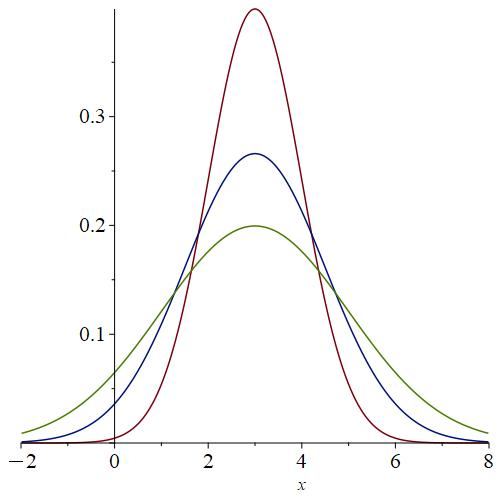
\includegraphics[width=0.7\textwidth]{Billeder/sammemiddel.jpg}
\end{center}
\begin{enumerate}[label=\roman*)]
	\item Hvad er middelværdien for de tre stokastiske variable?
	\item Hvilken stokastisk variabel har størst og mindst spredning?
\end{enumerate}

\section*{Opgave 3 (Uden Maple)}

En normalfordelt stokastisk variabel $X$ har følgende Gauss-kurve som tæthedsfunktion.
\begin{center}
	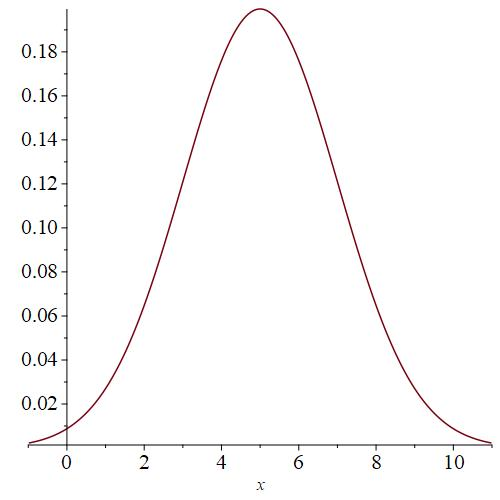
\includegraphics[width=0.7\textwidth]{Billeder/gauss.jpg}
\end{center}
Den har middelværdi $\mathbb{E}[X] = 5$. Det oplyses, at der for tæthedsfunktionen $f$ på figuren gælder, at
\begin{align*}
	\int_2^5f(x)dx = 0.433.
\end{align*}
Brug dette til at bestemme følgende sandsynligheder
\begin{enumerate}[label=\roman*)]
	\item $P(2<X<8)$.
	\item $P(X<2)$.
	\item $P(5<X)$.
	\item $P(8<X)$.
	\item $P(X=5)$.
\end{enumerate}




\section*{Opgave 4 (Uden Maple)}

En fordelingsfunktion for en normalfordelt stokastisk variabel $X\sim N(\mu,\sigma)$ ser ud som følgende.
\begin{center}
	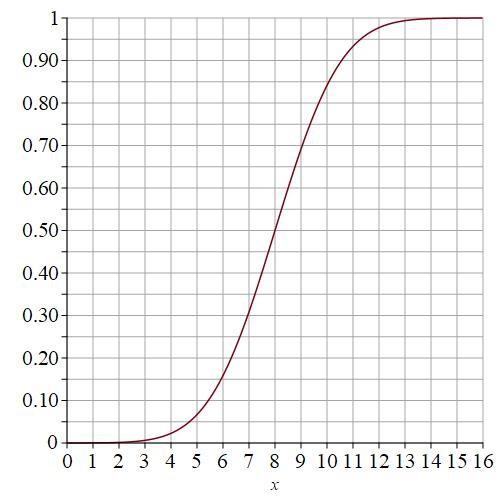
\includegraphics[width=0.7\textwidth]{Billeder/fordeling.jpg}
\end{center}
\begin{enumerate}[label=\roman*)]
	\item Bestem middelværdien $\mu$. 
	\item Bestem $P(X<7)$.
	\item Bestem $P(6<X<10)$. 
	\item Bestem $P(9<X)$.
	\item Bestem et $95\%$-konfidensinterval for middelværdien $\mu$. (Dette giver i princippet ikke mening, men humour me).
\end{enumerate}

\section*{Opgave 5 (Med Maple)}

I en bestemt pose lakridser er antallet af lakridser normalfordelt med middelværdi 103.5 og spredning 2.12. 
\begin{enumerate}[label=\roman*)]
	\item Bestem sandsynligheden for, at der i en pose er mindre end 99 lakridser. 
	\item Bestem sandsynligheden for, at der i en pose er mellem 102 og 105 lakridser. 
\end{enumerate}

\section*{Opgave 6 (Uden Maple)}

Her er tre tæthedsfunktioner og deres tilhørende fordelingsfunktioner for tre normalfordelte stokastiske variable med samme middelværdi og forskellig spredning. 
\begin{center}
	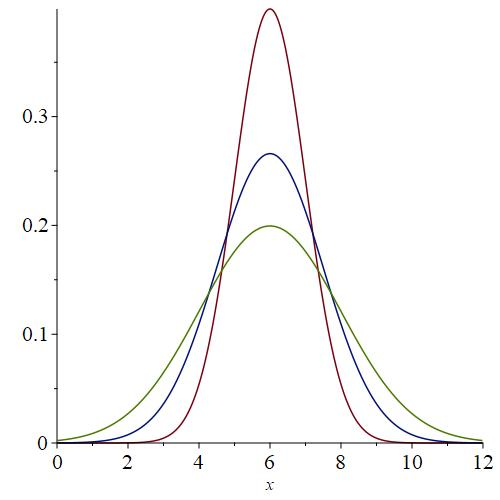
\includegraphics[width=0.45\textwidth]{Billeder/3gauss.jpg}
	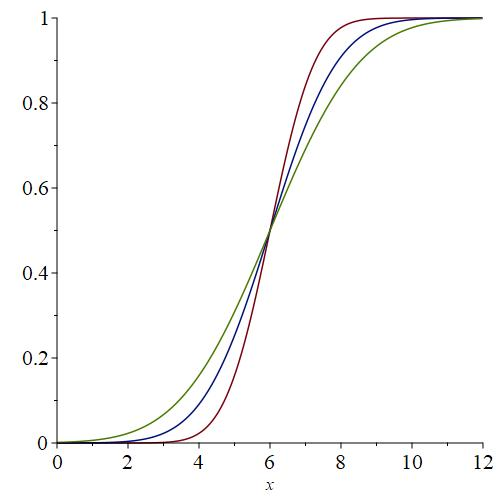
\includegraphics[width=0.45\textwidth]{Billeder/3fordeling.jpg}
\end{center}
